\documentclass{article}

\title{P02-FileSystem Report}
\date{29/11/2017}
\author{150008859}

\setlength{\parskip}{1em}
\setlength{\parindent}{0em}

\usepackage{listings}
\usepackage{amsmath,amssymb,amsthm}
\usepackage{mathtools}
\usepackage{graphicx}

\usepackage{graphicx}

\lstset{language=C}

\begin{document}
\maketitle
\newpage

\section{Introduction}

In this practical we implemented a file system.

My file system features the basic implementation. In addition, it features  multi level indexing with blocks (for file contents) and a LRU (Least Recently Used) cache (for file contents).

Finally, I built a small testing framework.

\section{Usage}

My implementation is not thread safe. To mount, run the following command.

\begin{lstlisting}[language=bash]
  ./myfs -d -s /cs/scratch/<username>/mnt
\end{lstlisting}

To run tests, first mount the filesystem then run the following commands.

\begin{lstlisting}[language=bash]
  cd testing
  chmod +x run_tests.sh
  ./run_tests.sh /cs/scratch/<username>/mnt
\end{lstlisting}

The command must be written exactly as mentioned, adding an extra slash at end of ``mnt'' may break my script.

\begin{lstlisting}
  
\end{lstlisting}

\section{Filesystem}

\begin{figure}[!htb]
  \caption{A visual representation of this file system}
  \center
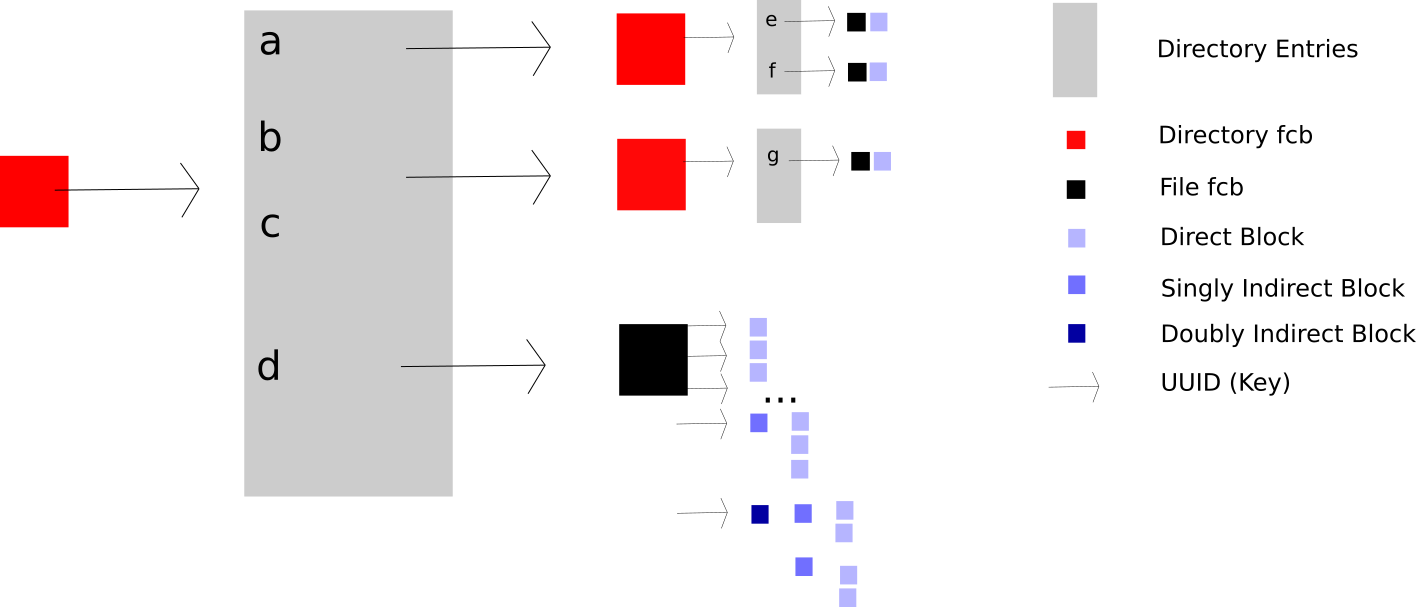
\includegraphics[scale=0.30]{images/diagram.png}
\end{figure}

\subsection{Directories}

A fcb may point to a directory. A directory fcb stores a key to its list of directory entries. A directory entry maps a filename to it's fcb. My implementation stores all the directory entries for a directory in a single entry in the database.

\subsection{Multi Level indexing and Blocks}

A fcb may point to a file. A multi level indexing scheme along with block storage is used to store files efficiently for retrieval. Instead of retrieving the entire contents of a file into memory, only the selected blocks required are read into memory. This scheme is vastly more efficient.

A block represents a unit of 4096 bytes. Each fcb stores keys to 13 direct blocks, a singly indirect block and a doubly indirect block. Each indirect block is capable of storing 256 keys ( block\_size / key\_size). This means the final doubly indirect block provides an additional $256^2$ blocks.

Blocks are added incrementally as space for storage is required. The direct blocks are filled up, followed by the singly indirect and finally the doubly indirect.

An indexing scheme is used to manipulate the blocks. This indexing scheme is used in conjuction with adding and removing blocks. This is used in the implementation of truncate to easily add or remove blocks.

\subsection{LRU Cache}

Blocks can be coupled with Caching.

A Least Recently Used caching scheme is deployed to reduce access times. In particular, this cache deals with temporal locality.

The Cache scheme operates on blocks containing file data.

When a request is made to retrieve a block from the database, the cache intervenes and handles the request. Changes are applied in the cache directly. When a cached block is ejected, the data is written to the database.

In order to implement the cache, I first implemented a queue and a hashtable (this can be found in myfs.h). 

The hashtable allows constant time lookups when trying to quickly find a cached block.

I implemented a hash function which seperates a uuid into 4 parts and ``exclusively ors'' them. This hash is converted into an index. Finally, the item is inserted into the bucket at that index.

The queue is a doubly linked list centred around a root node. 

When an object is requested, it may be cached. This is called a cache hit. During a cache hit, the cached block requested is moved to the front of the queue. Simialarly, during a cache miss, the data is cached and the new cache block is also moved to the front of the queue.

This process produces a queue where the least recently used cached block ends up at the back of the queue. When the cache is reaches its capacity, this cached block is evicted.

\subsection{Testing}

I have written a small testing framework in bash to test my implementation.

\begin{figure}[!htb]
  \caption{A graphic showing my tests running}
  \center
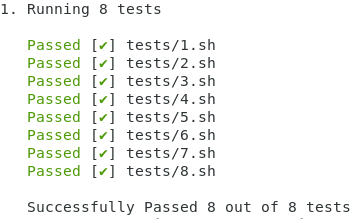
\includegraphics[scale=0.30]{images/tests.png}
\end{figure}

I have tested for the following.

\begin{itemize}
\item Multiple Directories, Multiple Sub Directories and the deletion
\item Verifying the contents of written data to a file (files in subdirectories) with enough data to test doubly indirect indexing
\item The creation of files, files in sub directories and the deletion
\item The truncation of files
\item Testing access/mod times
\item Testing chmod (I have also implemented chown, but is hard to test)
\end{itemize}

\section{Conclusion}

In conclusion, I found it intriguing to investigate schemes for reducing retrieval time. In particular, I enjoyed investigating the usage of multilevel indexing allowing data to be stored and retrieved in blocks as opposed to storing them in a single file. In addition, coupling this with caching to provide further increase in speed by dealing with temporal locality. Finally, I tested my implementation to verify it works.

\begin{thebibliography}{1}

\bibitem{LRU}
  LRU Cache
  \\\texttt{http://www.geeksforgeeks.org/lru-cache-implementation/}

\bibitem{Cache Replacement Policies}
  Cache Replacement Policies
  \\\texttt{https://en.wikipedia.org/wiki/Cache\_replacement\_policies}

\end{thebibliography}


\end{document}
